


%_______________
\newpage\subsection*{Exercises} % One-sample means with the t-distribution

% 1

\eoce{\qt{Identify the critical $t$\label{identify_critical_t}} An independent random 
sample is selected from an approximately normal population with unknown 
standard deviation. Find the degrees of freedom and the critical $t$-value 
(t$^\star$) for the given sample size and confidence level.
\begin{parts}
\item $n = 6$, CL = 90\%
\item $n = 21$, CL = 98\%
\item $n = 29$, CL = 95\%
\item $n = 12$, CL = 99\%
\end{parts}
}{}

% 2

\eoce{\noindent \begin{minipage}[c]{0.5\textwidth}
\qt{$t$-distribution\label{t_distribution}}
\textbf{\color{red}REQUIRES FINAL FORMATTING:
    move minipage outside of eoce environment.}
The figure on the right shows three 
unimodal and symmetric curves: the standard normal (z) distribution,  the $t$-
distribution with 5 degrees of freedom, and the $t$-distribution with 1 degree 
of freedom. Determine which is which, and explain your reasoning.
\end{minipage}
\begin{minipage}[c]{0.48\textwidth}
\begin{center}
\includegraphics[width=0.93\textwidth]{ch_inference_for_means/figures/eoce/t_distribution/t_distribution.pdf}
\end{center}
\end{minipage}
}{}

% 3

\eoce{\qt{Find the p-value, Part I\label{find_T_pval_1}} An independent random sample 
is selected from an approximately normal population with an unknown standard 
deviation. Find the p-value for the given set of hypotheses and $T$ test 
statistic. Also determine if the null hypothesis would be rejected at 
$\alpha = 0.05$.
\begin{parts}
\item $H_A: \mu > \mu_0 $, $n = 11$, $T = 1.91$
\item $H_A: \mu < \mu_0 $, $n = 17$, $T = -3.45$
\item $H_A: \mu \ne \mu_0 $, $n = 7$, $T = 0.83$
\item $H_A: \mu > \mu_0 $, $n = 28$, $T = 2.13$
\end{parts}
}{}

% 4

\eoce{\qt{Find the p-value, Part II\label{find_T_pval_2}} An independent random 
sample is selected from an approximately normal population with an unknown 
standard deviation. Find the p-value for the given set of hypotheses and $T$ 
test statistic. Also determine if the null hypothesis would be rejected at 
$\alpha = 0.01$.
\begin{parts}
\item $H_A: \mu > 0.5$, $n = 26$, $T = 2.485$
\item $H_A: \mu < 3$, $n = 18$, $T = 0.5$
\end{parts}
}{}

% 5

\eoce{\qt{Working backwards, Part I\label{work_backwards_1}} A 95\% confidence 
interval for a population mean, $\mu$, is given as (18.985, 21.015). This 
confidence interval is based on a simple random sample of 36 observations. 
Calculate the sample mean and standard deviation. Assume that all conditions 
necessary for inference are satisfied. Use the $t$-distribution in any 
calculations.
}{}

% 6

\eoce{\qt{Working backwards, Part II\label{work_backwards_2}} A 90\% confidence 
interval for a population mean is (65, 77). The population distribution is 
approximately normal and the population standard deviation is unknown. This 
confidence interval is based on a simple random sample of 25 observations. 
Calculate the sample mean, the margin of error, and the sample standard 
deviation.
}{}

% 7

\eoce{\qt{Sleep habits of New Yorkers\label{ny_sleep_habits}} New York is known as 
``the city that never sleeps". A random sample of 25 New Yorkers were asked how 
much sleep they get per night. Statistical summaries of these data are shown 
below. Do these data provide strong evidence that New Yorkers sleep less than 8 
hours a night on average?
\begin{center}
\begin{tabular}{rrrrrr}
 \hline
n   & $\bar{x}$ & s     & min   & max \\ 
 \hline
25  & 7.73      & 0.77  & 6.17  & 9.78 \\ 
  \hline
\end{tabular}
\end{center}

\begin{parts}
\item Write the hypotheses in symbols and in words.
\item Check conditions, then calculate the test statistic, $T$, and the 
associated degrees of freedom.
\item Find and interpret the p-value in this context. Drawing a picture may be 
helpful.
\item What is the conclusion of the hypothesis test?
\item If you were to construct a 90\% confidence interval that corresponded to 
this hypothesis test, would you expect 8 hours to be in the interval?
\end{parts}
}{}

% 8

\eoce{\qt{Heights of adults\label{adult_heights}} Researchers studying anthropometry 
collected body girth measurements and skeletal diameter measurements, as well as 
age, weight, height and gender, for 507 physically active individuals. The 
histogram below shows the sample distribution of heights in centimeters. 
\footfullcite{Heinz:2003} \\
\begin{minipage}[c]{0.75\textwidth}
\begin{center}
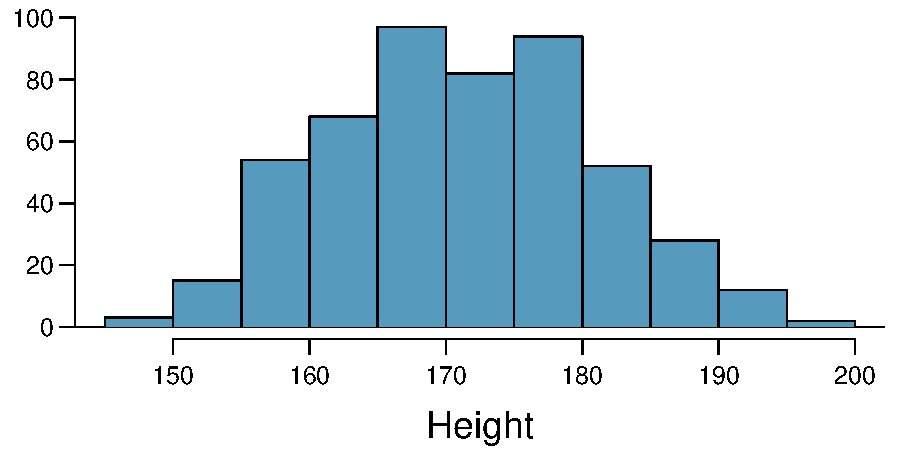
\includegraphics[width=\textwidth]{ch_inference_for_means/figures/eoce/adult_heights/adult_heights_hist.pdf}
\end{center}
\end{minipage}
\begin{minipage}[c]{0.23\textwidth}
\begin{center}
\begin{tabular}{l|r l}
Min     & 147.2 \\
Q1      & 163.8 \\
Median  & 170.3 \\
Mean    & 171.1 \\
SD      &  9.4 \\
Q3      & 177.8 \\
Max     & 198.1 \\
\end{tabular}
\end{center}
\end{minipage}
\begin{parts}
\item What is the point estimate for the average height of active individuals? 
What about the median?
\item What is the point estimate for the standard deviation of the heights of 
active individuals? What about the IQR?
\item Is a person who is 1m 80cm (180 cm) tall considered unusually tall? And is 
a person who is 1m 55cm (155cm) considered unusually short? Explain your 
reasoning.
\item The researchers take another random sample of physically active 
individuals. Would you expect the mean and the standard deviation of this new 
sample to be the ones given above? Explain your reasoning.
\item The sample means obtained are point estimates for the mean height of all 
active individuals, if the sample of individuals is equivalent to a simple 
random sample. What measure do we use to quantify the variability of such an 
estimate (Hint: recall that $SD_{\bar{x}} = \frac{\sigma}{\sqrt{n}}$)? Compute 
this quantity using the data from the original sample under the condition that 
the data are a simple random sample. 
\end{parts}
}{}

% 9

\eoce{\qt{Find the mean\label{find_mean}} You are given the following hypotheses:
\begin{align*}
H_0&: \mu = 60 \\
H_A&: \mu < 60
\end{align*}
We know that the sample standard deviation is 8 and the sample size is 20. For 
what sample mean would the p-value be equal to 0.05? Assume that all conditions 
necessary for inference are satisfied.
}{}

% 10

\eoce{\qt{$t^\star$ vs. $z^\star$\label{critical_t_vs_z}} For a given confidence 
level, $t^{\star}_{df}$ is larger than $z^{\star}$. Explain how $t^{*}_{df}$ 
being slightly larger than $z^{*}$ affects the width of the confidence interval.
}{}

% 11

\eoce{\qt{Play the piano\label{play_piano}} Georgianna claims that in a small city 
renowned for its music school, the average child takes less than 5 years of 
piano lessons. We have a random sample of 20 children from the city, with a 
mean of 4.6 years of piano lessons and a standard deviation of 2.2 years.
\begin{parts}
\item Evaluate Georgianna's claim using a hypothesis test.
\item Construct a 95\% confidence interval for the number of years students in 
this city take piano lessons, and interpret it in context of the data.
\item Do your results from the hypothesis test and the confidence interval 
agree? Explain your reasoning.
\end{parts}
}{}

% 12

\eoce{\qt{Auto exhaust and lead exposure\label{auto_exhaust_lead_exposure}} 
Researchers interested in lead exposure due to car exhaust sampled the blood of 
52 police officers subjected to constant inhalation of automobile exhaust fumes 
while working traffic enforcement in a primarily urban environment. The blood 
samples of these officers had an average lead concentration of 124.32 $\mu$g/l  
and a SD of 37.74 $\mu$g/l; a previous study of individuals from a nearby 
suburb, with no history of exposure, found an average blood level concentration 
of 35 $\mu$g/l.\footfullcite{Mortada:2000}
\begin{parts}
\item Write down the hypotheses that would be appropriate for testing if the 
police officers appear to have been exposed to a higher concentration of lead.
\item Explicitly state and check all conditions necessary for inference on 
these data.
\item Test the hypothesis that the downtown police officers have a higher lead 
exposure than the group in the previous study. Interpret your results in 
context.
%%% Note: solutions are also now commented out.
%\item Based on your preceding result, without performing a calculation, would a 99\% confidence interval for the average blood concentration level of police officers contain 35 $\mu$g/l? Explain why or why not.
\end{parts}
}{}

% 13

\eoce{\qt{Car insurance savings\label{car_insurance_savings}} A market researcher 
wants to evaluate car insurance savings at a competing company. Based on past 
studies he is assuming that the standard deviation of savings is \$100. He 
wants to collect data such that he can get a margin of error of no more than \$
10 at a 95\% confidence level. How large of a sample should he collect?
}{}

% 14

\eoce{\qt{SAT scores\label{sat_scores_CI}}
The standard deviation of SAT scores for students at
a particular Ivy League college is 250 points.
Two statistics students, Raina and Luke, want to estimate
the average SAT score of students at this college as part
of a class project.
They want their margin of error to be no more than 25 points.
\begin{parts}
\item
    Raina wants to use a 90\% confidence interval.
    How large a sample should she collect?
\item
    Luke wants to use a 99\% confidence interval.
    Without calculating the actual sample size, determine
    whether his sample should be larger or smaller
    than Raina's, and explain your reasoning.
\item
    Calculate the minimum required sample size for Luke.
\end{parts}
}{}
